\documentclass{article}
\usepackage{amsmath}
\usepackage{amssymb}
\usepackage{ctex}
\usepackage[margin=2cm]{geometry} % 设置较窄的边距使文档宽一些
\usepackage{multirow} % 支持表格中的多行单元格
\usepackage{graphicx} % 用于插入图片
\title{\heiti\zihao{2} 滑动摩擦系数测量}
\author{\songti author  Student ID  \\
课程号  XXXXXX.01 }
\date{2024.5.6}
\begin{document}
    \maketitle
\begin{abstract}
    本实验通过滑块与可调倾角平板的组合装置,测定了不同材质和工况下的静、动滑动摩擦系数。实验采用逐步调整平板倾角的方法,分别获得了最大静滑动摩擦力和动滑动摩擦力,并利用光电管测量滑块运动参数,结合理论公式进行数据处理和分析。实验结果表明,不同材质组合下的摩擦系数存在明显差异,验证了库伦摩擦定律的适用性。实验还培养了基本的数据处理能力和实验报告撰写能力。
    
    \noindent{\textbf{关键词:}摩擦系数,静摩擦,动摩擦,实验测量,数据分析}
\end{abstract} 
\section{引言}
摩擦现象广泛存在于自然界和工程实际中,对机械系统的能量损耗、运动控制等方面具有重要影响。滑动摩擦系数是表征物体接触界面摩擦特性的关键参数,通常分为静滑动摩擦系数和动滑动摩擦系数。由于摩擦机理复杂,理论计算难以精确,实验测定成为获取摩擦系数的主要手段。通过本实验,能够加深对滑动摩擦定律及其测量方法的理解,掌握实验数据的采集与处理流程,为后续相关研究和工程应用打下基础。 

\section{实验内容与设计}

\subsection{实验目的}
    \begin{enumerate}
        \item 了解滑动摩擦定律和静、动滑动摩擦系数的概念;
        \item 了解静、动滑动摩擦系数的测量原理和方法,测定并对比不同材质和工况下的静、
        动滑动摩擦系数;
        \item 实践基本的数据处理、分析以及书面报告表达。
    \end{enumerate}

\subsection{实验仪器}

    \begin{enumerate}
        \item JLT-1 理论力学多功能实验台;
        \item JLT-1 理论力学多功能实验台;
        \item 金属滑块、有机玻璃滑块;
        \item 不锈钢平板、铝合金平板。
    \end{enumerate}



\subsection{实验原理}
当两个相互接触的物体具有相对滑动趋势时,
在其接触界面处会产生阻碍相对运动的相互作用力,
这种力被定义为滑动摩擦力(Sliding friction force)。
滑动摩擦力的作用方向始终与接触面间的相对滑动趋势方向相反。
根据相对滑动趋势的发展程度,滑动摩擦力可处于静,动两种状态:
(1)当相对滑动趋势较小时,物体间保持相对静止状态,
此时产生的摩擦力称为静滑动摩擦力(Static sliding friction force)。
在此阶段,静滑动摩擦力的大小随外部作用力的增加而相应增大;
(2)当静滑动摩擦力达到其极限值而无法继续平衡外部作用力时,
物体间开始产生相对滑动,此时接触面间的摩擦力转变为动滑动摩擦力
(Kinetic sliding friction force)。
静滑动摩擦力所能达到的极限值被称为最大静滑动摩擦力
(Maximum static sliding friction force)。
由于除极限值以外的静滑动摩擦力不具有对物体接触界面状态的表征意义,
因此最大静滑动摩擦力常省略"最大"二字,简称为静滑动摩擦力。

库伦摩擦定律(Coulomb's law of friction)表明:当两物体相互滑动,
两物体间滑动摩擦力(记作 $F_d$ )正比于两物体接触处的正压力(记作 $N$ ),
即,$F_d=f_d \cdot N$ ,摩擦力方向与速度方向相反。
式中无量纲的系数 $f_d$ 称为动滑动摩擦系数,它与相对滑动速度无关,
仅取决于两物体接触面的材质与表面情况。
处于静-动临界状态的最大静滑动摩擦力(记作 $F_{\text {max }}$ )
同样仅取决于正压力和两物体接触面材质与表面情况,
因此可以相同形式描述:$F_{\max }=f_s \cdot N$ ,
式中无量纲的系数 $f_s$ 称为静滑动摩擦系数。    

依据摩擦理论,对于相同的两物体及其接触面状态,两滑动摩擦系数 $\left(f_d, ~ f_s\right)$ 应保持为常数。
由于摩擦的机理涉及接触面复杂的弹塑性变形乃至微观层面的分子作用,
人们很难通过现有理论准确计算出滑动摩擦系数,
一般需要借助实验方法进行近似测定。

本实验通过滑块和可调倾角的平板来测定物体的静,动滑动摩擦系数。
实验装置如图 1 所示。(最大)静滑动摩擦系数和动滑动摩擦系数的测量原理如下:

\subsection{(最大)静滑动摩擦系数测量}
预先设置较大的平板坡度,使滑块可以在平板上顺利下滑。通过升降手柄逐步降低平板倾斜角 $\varphi$ ,直至滑块保持静止,记录此时的平板倾斜角 $\varphi_s$ 。根据力的平衡有:

$$
\left\{\begin{array}{l}
F_{\max }=G \cdot \sin \varphi_s \\
N=G \cdot \cos \varphi_s
\end{array} \Rightarrow f_s=\frac{F_{\max }}{N}=\tan \varphi_s\right.
$$

\begin{figure}[h!]
    \centering
    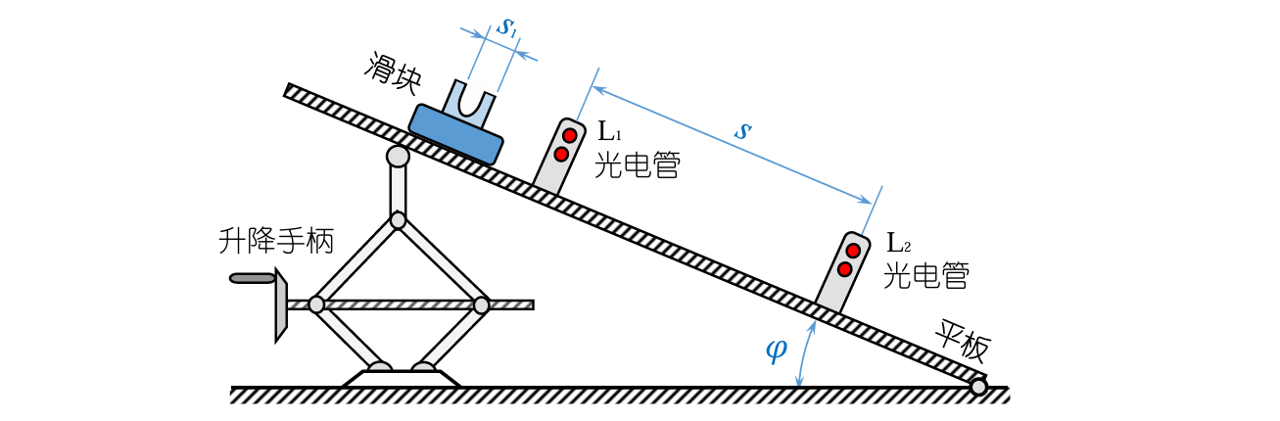
\includegraphics[width=\textwidth]{image/滑动摩擦系数测量装置示意图.png}
    \caption{滑动摩擦系数测量装置示意图}
\end{figure}

\subsection{动滑动摩擦系数的测量}

取倾斜角度 $\varphi>\varphi_s$ ,使得滑块可顺畅滑到平板底部。倾斜平板上有光电管 L1 和 L2,可检测固定于滑块上的相距 $s_1$ 的两挡板的抵达时间。测得两挡板相继扫过 L1 的时间间隔为 $t_1$ ,相继扫过 L 2 的时间间隔为 $t_2$ ,挡板最前锋扫过 L 1 和 L 2 的时间间隔为 $t_3$ ,那么,$s_1$ 中点通过 L1 和 L2 的时间间隔可近似表示为 $t_4=t_3+0.5\left(t_2-t_1\right)$ 。由此可计算得到滑块的平均加速度:

$$
a=\frac{V_2-V_1}{t_4}=\frac{\frac{s_1}{t_2}-\frac{s_1}{t_1}}{t_4}=\frac{s_1 \cdot\left(t_1-t_2\right)}{t_1 \cdot t_2 \cdot t_4}
$$


根据牛顿第二定律:

$$
\begin{gathered}
\left\{\begin{array} { l } 
{ \text { 平板切向:} \sum F _ { \tau } = m a } \\
{ \text { 平板法向:} \sum F _ { n } = 0 }
\end{array} \Rightarrow \left\{\begin{array}{l}
m g \sin \varphi-f_d \cdot N=m a \\
m g \cos \varphi-N=0
\end{array}\right.\right. \\
\Rightarrow \quad f_d=\frac{m g \sin \varphi-m a}{m g \cos \varphi}=\tan \varphi-\frac{a}{g \cos \varphi}
\end{gathered}
$$


将加速度代入,得到动滑动摩擦系数:

$$
f_d=\tan \varphi-\frac{s_1 \cdot\left(t_1-t_2\right)}{g \cdot t_1 \cdot t_2 \cdot t_4 \cdot \cos \varphi}
$$


    
\section{实验步骤}
% 简要描述实验的主要步骤
\subsection{三线摆测规则圆盘的转动惯量}
\begin{enumerate}
    \item % 步骤 1
    \item % 步骤 2
    % ...
\end{enumerate}

\subsection{三线摆测不规则物体的转动惯量}
\begin{enumerate}
    \item % 步骤 1
    \item % 步骤 2
    % ...
\end{enumerate}

\section{实验数据处理}
\subsection{三线摆测规则圆盘的转动惯量}
\subsubsection{实验原始数据}
% 在此处插入原始数据表格
% \begin{table}[h!]
%     \centering
%     \renewcommand{\arraystretch}{1.5}
%     \setlength{\tabcolsep}{8pt}
%     \begin{tabular}{|c|c|c|c|c|c|}
%     \hline
%     % 表头
%       &    &    &    &    &    \\ \hline
%       &    &    &    &    &    \\ \hline
%       &    &    &    &    &    \\ \hline
%     \end{tabular}
%     \caption{实验原始数据表}
%     \label{tab:raw_data}
% \end{table}

% 如有需要,可插入图片
% \begin{figure}[h!]
%     \centering
%     \includegraphics[width=0.5\textwidth]{example.png}
%     \caption{实验相关图片}
%     \label{fig:example}
% \end{figure}

% 如有需要,可插入并排图片
% \begin{figure}[h!]
%     \centering
%     \begin{minipage}{0.48\textwidth}
%         \centering
%         \includegraphics[width=\textwidth]{example1.png}
%         \caption{实验相关图片}
%         \label{fig:example1}
%     \end{minipage}
%     \hfill
%     \begin{minipage}{0.48\textwidth}
%         \centering
%         \includegraphics[width=\textwidth]{example2.png}
%         \caption{实验相关图片}
%         \label{fig:example2}
%     \end{minipage}
% \end{figure}



 
\section{思考题}
\subsection{分析本实验的误差,并简述如何减少误差。}
实验的误差的来源:
\begin{enumerate}
    \item \textbf{摩擦面污染:} 摩擦面的污染,如灰尘、油污、产生的铝屑等,可能导致摩擦力的增加或减少,从而引入误差。
    
    \item \textbf{测量误差:} 倾斜角度,长度的测量
    
    \item \textbf{表面粗糙度不一致:} 不同材料的表面可能存在微小的瑕疵或不均匀性,影响摩擦系数的测量。
    
    \item \textbf{外部干扰:} 滑块与玻璃壁面的接触产生的摩擦
    \item \textbf{实验操作不一致:} 实验过程中防止位置的不同,导致速度不同,影响摩擦系数的测量。
\end{enumerate}
减少误差的方法:
\begin{enumerate}
    \item \textbf{清洁摩擦面:} 在实验前,确保摩擦面清洁,去除灰尘、油污等污染物。
    
    \item \textbf{精确测量:} 使用高精度的测量工具,确保倾斜角度和长度的测量准确。
    
    \item \textbf{控制环境:} 在相对恒定的温度和湿度下进行实验,以减少外部环境对摩擦系数的影响。
    
    \item \textbf{多次实验取平均值:} 进行多次实验,取平均值以减少偶然误差的影响。
    
    \item \textbf{标准化操作:} 确保每次实验操作一致,如施加力的方式、速度等,以提高结果的可重复性。
    
\end{enumerate}
\subsection{物体从静止到滑动的过渡阶段出现"黏滑现象"(即间歇性滑动),
试分析可能的原因及其对摩擦系数测量精度的影响。}
可能的原因有:
\begin{enumerate}
    \item \textbf{表面不规则性:} 物体表面可能存在微小的不规则性或粗糙度,这会导致接触面之间的间隙不均匀。在外力作用下,物体表面某些部分可能首先发生滑动,而其他部分则可能由于微小的表面不平整而维持静止。这种不均匀的滑动会导致间歇性滑动现象。
    
    \item \textbf{粘附力:} 当物体在开始滑动之前,表面之间的微小接触点可能会形成短暂的粘附力。在外力的作用下,这些粘附点可能会突然断裂,从而导致滑动。这种突然的“粘附 - 断裂”循环会表现为间歇性滑动。
    
    \item \textbf{摩擦系数变化:} 物体的摩擦系数不是恒定的,特别是在滑动开始时,摩擦系数可能发生较大波动。起初,表面可能有较高的静摩擦力,需要克服较大的力才能开始滑动,而一旦克服这些力后,表面会转为动态摩擦,摩擦力可能突然减小。这种摩擦力的波动可能导致间歇性滑动。
    
    \item \textbf{外部干扰:} 施加的外力如果不均匀(如外力波动或施力方向变化)也会导致物体滑动的不稳定,从而引发间歇性滑动。
\end{enumerate}

对摩擦系数测量精度的影响:
\begin{enumerate}
    \item \textbf{误差增加:} 黏滑现象使得摩擦力的变化不再平滑,测量过程中可能出现间歇性增大或减小的摩擦力波动,这样的波动会导致摩擦系数测量的不稳定性,从而使得测量结果的准确性降低。
    
    \item \textbf{测量困难:} 在黏滑现象发生时,无法简单地通过持续的滑动来测量摩擦系数,可能需要多次测量或更复杂的实验设计来得到一个较为准确的值。否则,得出的摩擦系数可能仅代表一个平均值,而不是真正的动态摩擦系数。
    
    \item \textbf{摩擦模型的适用性:} 黏滑现象可能表明传统的静摩擦和动摩擦模型不再适用。许多经典摩擦模型假设摩擦力是连续变化的,而黏滑现象则表明摩擦力可能会出现突变或不稳定的变化,这会使得基于这些模型的计算变得不可靠。
\end{enumerate}


\subsection{根据实验结果讨论是否有以下相关性:动摩擦系数小的材料,
其静,动摩擦系数也接近;动摩擦系数大的材料,
其静,动摩擦系数差距也大。}

根据实验结果,我们可以猜测:
\begin{enumerate}
    \item \textbf{动摩擦系数小的材料,静、动摩擦系数接近} 动摩擦系数较小的材料通常表明其表面粗糙度较小或材料间的分子间力较弱。对于这种材料,静摩擦和动摩擦的差距可能较小,因为当开始滑动时,材料之间的摩擦力不会发生剧烈变化。通常情况下,摩擦力从静摩擦转变为动摩擦时,变化较为平缓,因此静摩擦系数和动摩擦系数较接近。
    
    \item \textbf{动摩擦系数大的材料,静、动摩擦系数差距大} 动摩擦系数较大的材料通常意味着表面粗糙度较高或材料间存在较强的分子间力。在这种情况下,静摩擦系数和动摩擦系数的差距可能较大。静摩擦需要克服初始的粘附力和微小不规则性,而一旦开始滑动,摩擦力变化较为剧烈。因此,材料的静摩擦系数可能显著高于动摩擦系数,导致两者之间的差距较大。
    
\end{enumerate} 
\section{总结}
本实验通过对不同材质滑块与平板的摩擦系数测定,验证了库伦摩擦定律的基本规律。实验结果显示,静滑动摩擦系数普遍大于动滑动摩擦系数,不同材料组合下的摩擦系数差异明显。实验过程中,掌握了摩擦系数的测量原理、实验操作方法及数据处理技巧。通过本次实验,不仅加深了对摩擦现象本质的理解,也提升了实验设计与分析能力,为今后相关实验和理论研究提供了有益的参考。 

\section{参考文献}

[1] 理论力学实验指导书 [M] . 北京大学出版社,2007 

[2] 王惠明。应用理论力学实验 [M] . 北京高等教育出版社,2009

[3] 宋保江,阎绍泽。界面黏滑摩擦现象的研究进展 [J].中国机械工程,2017,28(13):1513-1522.
 



\end{document}